\documentclass[a4paper, 11pt, draft]{article}

\usepackage[numbers]{natbib}

\usepackage{amsmath,amssymb,amsthm}

\usepackage[retainorgcmds]{IEEEtrantools}


\usepackage{pgfplots}

\usepackage{enumitem}

\usepackage{booktabs}

\usepackage{subcaption}

\usepackage{graphicx}

\usepackage{minted}


%\usepackage[adobe-utopia]{mathdesign}
%\usepackage{zi4}

\usepackage[T1]{fontenc}
\usepackage[utf8]{inputenc}

\usepackage{lmodern}

%\usepackage{microtype}

\newtheorem{theorem}{Theorem}
\newtheorem*{th_recall_contrib_sc}{Theorem \ref{th:contrib:sc}}
\newtheorem*{th_recall_expect}{Theorem \ref{th:expect}}
\newtheorem*{lemma}{Lemma}

\newlist{algosteps}{enumerate}{10}
\setlist[algosteps]{label*=\arabic*.}

% macros
\newcommand{\peersim}{PeerSim}

\newcommand{\deccen}{\textsc{Deccen}}
\newcommand{\multibfs}{\textsc{Multi-BFS}}

\newcommand{\mdisc}{\textsf{{\footnotesize DIS\-COV\-E\-RY}}}
\newcommand{\mdiscargs}[3]{\mdisc$\langle #1,#2,#3, \sigma_{#1 #2} \rangle$}
\newcommand{\mdiscargsfull}[4]{\mdisc$\langle #1,#2,#3, #4 \rangle$}
\newcommand{\mdiscstart}[1]{\mdisc$\langle #1,#1,0,1 \rangle$}
\newcommand{\mrep}{\textsf{{\footnotesize REPORT}}}
\newcommand{\mrepargs}[2]{\mrep$\langle #1,#2, \delta(#1|#2), \sigma(#1|#2), \sigma_{#1 #2} \rangle$}
\newcommand{\mrepleaf}[2]{\mrep$\langle #1,#2, 0, 0, \sigma_{#1 #2} \rangle$}
\newcommand{\mdecrepargs}[2]{\mrep$\langle (#1,#2), \sigma_{#1 #2}, d_{#1 #2}\rangle$}
\newcommand{\mdecrepargsfull}[3]{\mrep$\langle (#1,#2), \sigma_{#1 #2}, #3\rangle$}

\newcommand{\swait}[1]{\textsf{{\footnotesize WAITING}}$(#1)$}
\newcommand{\sact}[1]{\textsf{{\footnotesize ACTIVE}}$(#1)$}
\newcommand{\scomp}[1]{\textsf{{\footnotesize COMPLETED}}$(#1)$}


\title{Peer-to-Peer Systems}
\author{Andrea Maggiordomo -- \texttt{mggndr89[at]gmail.com} \\[1mm] Laurea Magistrale in Informatica, Universit\`a di Pisa}
\date{2016}

\begin{document}
\maketitle

% !TeX root = p2p.tex

\theoremstyle{definition}
\newtheorem*{defcc}{Closeness centrality}
\newtheorem*{defsc}{Stress centrality}
\newtheorem*{defbc}{Betweenness centrality}

\section{Introduction}

The task of the project was to define \deccen{}, a decentralized algorithm to compute stress centrality indices in a network based on the ideas introduced in \cite{lehmann2003}, and study its behavior using the \peersim{} simulator \cite{peersim}. Additionally -- given the high cost of the algorithm -- approximation techniques could be proposed in order to reduce the communication overhead and memory requirements, and the algorithm could be extended to also compute the closeness and betweenness centrality indices.

This report defines a version of \deccen{} capable of computing all the three centrality measures mentioned. Furthermore, a different decentralized algorithm is defined, based on the previous works of Brandes, and Eppstein and Wang \cite{brandes2001, ew2004, brandes2007}, to approximate centrality values by sampling a limited amount of network nodes. This second algorithm, referred to as \multibfs{}, has a significantly smaller communication overhead than \deccen{}.

This document is organized as follows: in section \ref{sec:def} some preliminary definitions are given, while \deccen{} is defined in section \ref{sec:deccen} and \multibfs{} is defined in section \ref{sec:mbfs}. Experimental results are shown in section \ref{sec:exp}: the aims of the experiments were to compare the performance of the two algorithms, and to evaluate the quality of the estimates obtained with \multibfs{}. Follow a small overview of the most relevant choices made in the development of the project code, and the proofs of some results introduced in section \ref{sec:mbfs}.


\section{Preliminary definitions and assumptions}
\label{sec:def}

The task is to compute centrality indices for a given undirected graph $G = (V,E)$, which is assumed to be connected. Unless otherwise stated, $n$ denotes the number of nodes $|V|$ and $m$ the number of edges $|E|$. Each vertex $v \in V$ represents a network node with some given computational power, that can only communicate with its direct neighbors $N_v = \{u \in V : \{u,v\} \in E\}$. The terms \emph{vertex} and \emph{node} will be used interchangeably.

A \emph{path} of \emph{length} $k$ from a source $s \in V$ to a destination $t \in V$ is a sequence $\langle v_0, v_1, \dots, v_k \rangle$ of vertices such that $s=v_0$, $t=v_k$ and $\{v_{i-1}, v_i\} \in E$ for $i = 1,2,\dots,k$. The \emph{distance} $d(u,v)$ between two vertices is the length of the shortest path that connects them (with $d(u,u) = 0$) while the diameter $\Delta$ is the maximum distance between any pair of vertices. Note that $d(u,v) = d(v,u)$ since the graph is undirected. A vertex $v$ is a \emph{predecessor} of $w$ with respect to $s$ if $\{v,w\} \in E$ and $d(s,v) +1 = d(s,w)$. The \emph{predecessor set} $P_s(w)$ of a vertex $w$ is the set of all predecessors of $w$ with respect to $s$.

The number of different shortest paths that connect two vertices $s,t \in V$ is denoted by $\sigma_{st}$, while the quantity $\sigma_{st}(v)$ is the number of shortest paths between $s$ and $t$ that pass through $v$ (this means that if $v = s$ or $v = t$ then $\sigma_{st}(v)$ is always zero).

The centrality indices relevant to this document are the following:
\begin{defcc} The \emph{closeness} centrality $C_C(v)$ of a vertex $v \in V$ is
\begin{equation}
 C_C(v) = \frac{\sum_{u \in V} d(u,v)}{n-1}
\end{equation}
\end{defcc}
\begin{defsc} The \emph{stress} centrality $S_C(v)$ of a vertex $v \in V$ is
\begin{equation}
 S_C(v) = \sum_{s \in V} \sum_{t \in V} \sigma_{st}(v)
\end{equation}
\end{defsc}
\begin{defbc} The \emph{betweenness} centrality $B_C(v)$ of a vertex $v \in V$ is
\begin{equation}
 B_C(v) = \sum_{s \in V} \sum_{t \in V} \frac{\sigma_{st}(v)}{\sigma_{st}}
\end{equation}
\end{defbc}

The algorithms described in this report all assume an underlying syn\-chro\-nous communication model where the computation evolves in steps: at each step all the network nodes perform their computations independently and autonomously, and the messages they send at step $t$ are delivered to the destinations and processed at step $t+1$.
% !TeX root = p2p.tex

\newcommand{\mdecrepargs}[2]{\mrep$\langle (#1,#2), \sigma_{#1 #2}, d_{#1 #2}\rangle$}
\newcommand{\mdecrepargsfull}[3]{\mrep$\langle (#1,#2), \sigma_{#1 #2}, #3\rangle$}

The specification of \deccen{} is based on the algorithmic scheme outlined in \cite{lehmann2003}. Initially, each node broadcasts itself on the network. Exploiting the synchronous model, after $k$ steps any node $t \in V$ will know all the nodes $s \in V$ such that $d(s,t) = k$ and the number of shortest paths  $\sigma_{st}$ that links it to each of them. This information is stored locally and also reported in broadcast to allow other nodes $v \in V$ to compute the quantity $\sigma_{st}(u)$ necessary to compute the betweenness and stress centrality indices. The value $\sigma_{st}(u)$ can be determined by exploiting the following

\begin{lemma}[Bellman conditions]
A node $v \in V$ lies on a shortest path from $s \in V$ to $t \in V$ if and only if $d(s,t) = d(v,s) + d(v,t)$.
\end{lemma}

The synchronous model ensures that if a node $v$ lies on a shortest path between $s$ and $t$ and receives a report for such a pair, it has already computed $\sigma_{vs}$ and $\sigma_{vt}$. Then, according to the above conditions $\sigma_{st}(v) = \sigma_{vs} \cdot \sigma_{vt}$.

\subsection{Message types}

\paragraph{\mdiscargs{s}{u}{d}} These messages are used to track distances and the number of shortest paths from a specific origin. They contain the source $s \in V$ of the broadcast, the sender $u \in V$, the distance $d = d(s,u)$ of $u$ from $s$ and the number of shortest path that connect $u$ to $s$.

\paragraph{\mdecrepargs{s}{t}} These messages are broadcast by $t$ after having determined the number of shortest paths to $s$ and the distance from it.

\subsection{Node state}

Each node $v$ maintains three accumulators $C_C$, $C_B$ and $C_S$ for closeness, betweenness and stress centrality (the closeness centrality will be retrieved as $1/C_C$), a set $R$ of node pairs for which a \mrep{} message has already been received, and two dictionaries $D$ and $S$ that associate each node $s \in V$ with the discovered distance $d(s,v)$ and the number of shortest paths $\sigma_{sv}$ respectively.

\subsection{Protocol initialization}

Each node $v \in V$ initializes the accumulators $C_C$, $C_B$ and $C_S$ to $0$, the set $R$ to the empty set, the dictionary $D$ so that it only contains the entry $(v,0)$ and $S$ so that it only contains the entry $(v,1)$. Furthermore, it sends to all its neighbors a \mdiscstart{v} message.

\subsection{Step actions}
The processing performed by each node $v$ at each step is the following:

\begin{algosteps}

  \item All the \mdisc{} messages having a source $s$ for which the dictionary $D$ contain no mapping are grouped together. (These will be the nodes ``discovered'' at this step).

  \item Each group of messages is processed independently. For each group, let $s$ be the source and $d$ be the distance of all the \mdiscargs{s}{u}{d} messages in it (these will be the same for all the messages), then:
  \begin{algosteps}
    \item Add the entry $(s,d+1)$ to the dictionary $D$, so that $D[s] = d+1$.
    \item Let $\sigma_{sv} = \sum_{u} \sigma_{su}$ and add the entry $(s,\sigma_{sv})$ to  $S$. (The number of shortest paths from $s$ to $v$ is the sum of the number of shortest paths from $s$ to all the predecessors of $v$).
    \item Send a \mdecrepargsfull{s}{v}{d+1} message to each neighbor node.
  \end{algosteps}
  
  \item For each \mdecrepargs{s}{t} message such that $(s,t) \notin R$:
  \begin{algosteps}
    \item If $s = v$ then $C_C \gets C_C + d_{st}$.
    \item If $d_{st} = D[s]+D[t]$ let $\sigma_{st}(v) = \sigma_{sv} \cdot \sigma_{tv}$, then $C_B \gets \frac{\sigma_{st}(v)}{\sigma_{st}}$ and $C_S \gets \sigma_{st}(v)$.
    \item Add the pair $(s,t)$ to the set $R$, and forward the \mrep{} message to all the neighbors.
  \end{algosteps}
\end{algosteps}

\subsection{Cost analysis}
The broadcast of a \mdisc{} or a \mrep{} requires $O(m)$ messages. Since each nodes starts a \mdisc{} and generates $n-1$ reports the total number of messages exchanged is $O(nm + n^2m)$, with \mrep{} messages inducing the dominant factor $n^2m$.

In terms of memory consumption, each node will add $O(n)$ entries each of the two dictionaries and $O(n^2)$ pairs to the set $R$.

% !TeX root = p2p.tex

\section{Approximation of centrality indices}

The main issue with the \deccen{} algorithm is its computational cost both in terms of memory consumption and number of messages exchanged, rendering the algorithm impractical for networks of reasonable size.. In order to keep track of the forwarded report messages and guarantee the termination of the protocol each node needs to maintain a data structure of size $O(n^2)$, while the number of messages exchanged is $O(n^2m)$.

However, if we are for example interested in computing centrality indices in order to mitigate network congestion a simple estimation of the values could be sufficient. In the following I propose an approximation algorithm that adapts an idea originally developed for closeness centrality in \cite{ew2004} and expanded for the estimation of betweenness centrality in \cite{brandes2007}. The idea is to isolate the contribution of a single node $s$ to the centrality values of all the other nodes in the network and compute those contributions by solving a Single-Source-Shortest-Path problem starting from $s$. We can then compute the centrality of a node $v$ by adding the contributions of all the other nodes to $v$ (that is, by solving $n$ SSSP instances starting from all the nodes and accumulating the contributions locally). In our case, the SSSP problem is converted to a decentralized Breadth First Search.

The approximation algorithms described in \cite{ew2004,brandes2007} estimate the centrality values by solving the SSSP problems for a restricted set of source nodes.

\subsection*{Contribution of a source to Closeness centrality}

The contribution of a source $s$ to the closeness centrality value of $v$ is simply the distance $d(s,v)$ of $v$ from $s$:

\begin{equation}
\gamma(s|v) = d(s,v) .
\end{equation}

\subsection*{Contribution of a source to Betweenness centrality}

The contribution of a source $s$ to the betweenness centrality of $v$ is the \emph{dependency} of $s$ on $v$ introduced in \cite{brandes2001}:

\begin{equation}
\delta(s|v) = \sum_{t \in V} \frac{\sigma_{st}(v)}{\sigma_{st}},
\end{equation}
that allows to rewrite the betweenness centrality of $v$ as

\begin{equation*}
BC(v) = \sum_{s \in V} \delta(s|v).
\end{equation*}

\subsection*{Contribution of a source to Stress centrality}

The contribution to stress centrality is analogous to the betweenness centrality:

\begin{equation} \label{eq:contrib:sc}
\sigma(s|v) = \sum_{t \in V} \sigma_{st}(v),
\end{equation}
and the stress centrality of $v$ is rewritten as

\begin{equation*}
SC(v) = \sum_{s \in V} \sigma(s|v).
\end{equation*}

\subsection{Computing contributions from a single source}
\label{sec:recursive}

As stated previously, a decentralized Breadth First Search can be adapted to compute the contribution of a source to any of the three centrality indices considered. The closeness centrality contribution is simply the distance from the source to the node (that is, the depth of the visited node in the Breadth-First tree) and it can be computed directly during the visit.

For betweenness centrality, \cite{brandes2001} shows that dependencies of a source obey a recursive relation expressed in terms of predecessors set:
\begin{theorem}[Brandes, 2001]
\label{th:contrib:bc}
The dependency of $s \in V$ on any $v \in V$ obeys
\begin{equation} \label{eq:th:contrib:bc}
\delta(s|v) = \sum_{w : v \in P_s(w)} \frac{\sigma_{sv}}{\sigma_{sw}} \cdot (1 + \delta(s|w)) .
\end{equation}
\end{theorem}
For stress centrality contributions a similar relation holds (the proof is reported in the appendix):
\begin{theorem}
\label{th:contrib:sc}
The stress centrality contribution of $s \in V$ on any $v \in V$ obeys
\begin{equation} \label{eq:th:contrib:sc}
\sigma(s|v) = \sum_{w : v \in P_s(w)} \sigma_{sv} \cdot \left( 1 + \frac{\sigma(s|w)}{\sigma_{sw}} \right) .
\end{equation}
\end{theorem}

The predecessor sets of all the nodes can be easily discovered by adjusting the ``descent'' phase of the BFS algorithm, while contributions are computed during a backward walk from the frontier of the BF-Tree back to the source.

\subsection{Random sampling of source nodes [FIXME]}

To let the algorithm operate in a decentralized way, each node independently initiates a visit with a given probability $p$, which reflects the fraction of the network sampled. Even if the number of samples is not known beforehand, eventually all the nodes will become aware of the number of sources that initiated a visit (let it be $k$).

The contributions of sample $v_i$ to the closeness, stress and betweenness centrality of any node $u$ can be modeled with the following random variables

To estimate the value of centrality indices, first the result of sampling from a source node $v_i$ at a node $u$ is modeled using the following random variables:
\begin{eqnarray*}
X_i(u) = \frac{n}{n-1} \cdot d(v_i,u) , \quad
Y_i(u) = n \cdot \delta(v_i|u) , \quad
Z_i(u) = n \cdot \sigma(v_i|u) ,
\end{eqnarray*}
then centrality indices are approximated with the following estimators:
\begin{eqnarray*}
\widehat{C}_C(u) = \sum_{i=1}^k \frac{X_i(u)}{k}, \quad
\widehat{C}_B(u) = \sum_{i=1}^k \frac{Y_i(u)}{k}, \quad
\widehat{C}_S(u) = \sum_{i=1}^k \frac{Z_i(u)}{k} .
\end{eqnarray*}

The derivations for the following theorem -- which ensures the estimators are unbiased -- are reported in the appendix.

\begin{theorem}[Unbiased estimators]
\label{th:expect}
The expected values of the centrality estimators are the exact centrality indices:
 \begin{enumerate}[label=\textup{(\alph*)}]
  \item $\mathbf{E}[\widehat{C}_C(u)] = C_C(u)$,
  \item $\mathbf{E}[\widehat{C}_S(u)] = C_S(u)$,
  \item $\mathbf{E}[\widehat{C}_B(u)] = C_B(u)$.
  \end{enumerate}
\end{theorem}

\subsection{Algorithm specification}

In this section the algorithm is detailed. The only parameter of the algorithm is the probability $p$ with which each independent node decides to begin a visit of the network. The network size $n$ is assumed to be known to all the agents in the network. Initially, every node sets to zero the estimation of each centrality index.

\subsubsection{Message types}

\paragraph{\mdiscargs{s}{u}{d}} Messages of this type are used during the descent from a source to build the predecessors sets at each node. Relevant fields are the source $s$ of the visit, the sender $u$, the distance $d$ of the sender to the source (that is, $d = d(s,u)$) and the number of shortest path from the source to the sender $\sigma_{su}$.

\paragraph{\mrepargs{s}{v}} These messages are sent by a node $v$ as part of the backtracking phase to inform its predecessors of the computed contributions and to allow them to compute their own by applying the recursive relations introduced in section \ref{sec:recursive}.

\subsubsection{Visit states}

Visit states are parametric with respect to the discovery from a source $s \in V$. A node $v$ is in state:
\begin{description}
\item[\swait{s}] if it has not yet received any \mdisc{} having $s$ as source.
\item[\sact{s}] if it has received one or more \mdisc{} messages with source $s$ and has not yet computed the contributions of $s$ to its centrality indices.
\item[\scomp{s}] if it has computed the contributions of $s$ to its centrality indices, updated them accordingly, and reported the contributions to each predecessor in $P_s(v)$ by sending the appropriate \mrep{} messages.
\end{description}

\subsubsection{Node state}
Each node $v$ maintains three centrality accumulators $C_C$, $C_B$ and $C_S$ like in \deccen{}, and a counter $k$ to track the number of sample nodes involved in the protocol.

Furthermore, while a node is in state \sact{s} when dealing with a visit from $s$ it will need to partition the set of neighbors $N_v$ in three subsets: the set of predecessors $P_s(v)$, the set of siblings $S_s(v)$ and the set of children $C_s(v)$, as well as track contributions of $s$ to its centrality scores with three parametric accumulators $C_C(s)$, $C_B(s)$ and $C_S(s)$.

\subsubsection{Protocol initialization}
Upon initialization, a node $v$ clears its centrality accumulators and the counter $k$, and enters state \swait{s} for all $s \in V$. Then, with probability $p$ initiates a visit by entering state \sact{v}, sending a \mdiscargsfull{v}{v}{0}{1} to every neighbor and letting $P_v(v) = \emptyset$.

\subsubsection{Step actions}
\label{multibfs:step}
The actions performed by a node $v$ at each step are the following:

\begin{algosteps}
  \item The messages received at the current step are divided by type and then \mdisc{} messages are grouped by source.
  \item For each group of \mdiscargs{s}{u}{d} messages having source $s$ and distance $d$ with $v$ in state \swait{s}:
  \begin{algosteps}
    \item Change state to \sact{s}, let $C_C(s) \gets d+1$, $C_B(s) \gets 0$, $C_S(s) \gets 0$, collect all the senders $u$ in the predecessor set $P_s(v)$. Let $\sigma_{sv} = \sum_{u \in P_s(v)} \sigma_{su}$.
    \item If $P_s(v) = N_v$ send a \mrepleaf{s}{v} message to all the predecessors $u \in P_s(v)$ and change state to \scomp{s}. 
    \item Otherwise, send to all $w \in N_v \setminus P_s(v)$ a \mdiscargs{s}{v}{d+1} message and change state to \sact{s}.
  \end{algosteps}
    \item For each group of \mdiscargs{s}{u}{d} messages having source $s$ and distance $d$ with $v$ in state \sact{s}:
    \begin{algosteps}
      \item Under the synchronous model assumption $v$ can only receive such messages from nodes $u$ such that $d(s,u) = d(s,v)$. Collect these nodes in the set $S_s(v)$ of the siblings of $v$ with respect to $s$. (Note that these messages are received exactly one step after $v$ has been contacted by its predecessors).
    \end{algosteps}
  \item For each \mrepargs{s}{w} message received with $v$ in state \sact{s}:
  \begin{algosteps}
      \item Add $w$ to the children set $C_s(v)$.
      \item Update $C_B(s) \gets C_B(s) + \frac{\sigma_{sv}}{\sigma_{sw}} \cdot (1 + \delta(s|w))$.
      \item Update $C_B(s) \gets C_B(s) + \sigma_{sw} \cdot ( 1 + \sigma(s|w)/\sigma_{sw} )$.
    \end{algosteps}
  \item For any $s \in V$ such that $v$ is in state \sact{s}, if $P_s(v) \cup S_s(v) \cup C_s(v) = N_v$ then:
  \begin{algosteps}
      \item If $s \neq v$ update the accumulators:
      \begin{itemize}
        \item[-] $C_C \gets C_C + C_C(s)$
        \item[-] $C_B \gets C_B + C_B(s)$
        \item[-] $C_S \gets C_S + C_S(s)$
      \end{itemize}
      and send a \mrepargs{s}{v} message to all the predecessors contained in $P_s(v)$.
      \item Increment the counter $k$ and change state to \scomp{s}.
    \end{algosteps}
\end{algosteps}
A node $v$ can obtain the value of the estimators in the following way:
\begin{eqnarray*}
\widehat{C}_C(v) =  \left( \frac{n}{k} \, C_C \right)^{-1}, \quad
\widehat{C}_B(v) = \frac{n}{k} \, C_B, \quad
\widehat{C}_S(v) = \frac{n}{k} \, C_S .
\end{eqnarray*}

Note that if the algorithm is executed with $p=1$ this is basically the decentralized version of the algorithm described in \cite{brandes2001}, and the estimators are actually the exact centrality indices.[FIXME move this at the beginning of the description]

\subsection{Cost analysis}

Each independent search requires $O(m)$ messages for the \mdisc{} phase and $O(m)$ messages to backtrack with \mrep{} messages. The parameter $p$ determines the fraction of nodes $pn$ that initiate a \mdisc{} search, so the total number of messages is $O(\lceil pn \rceil m)$.

In terms of memory consumption, note that for each $v \in V$ there are at most $\lceil pn \rceil$ other nodes $s$ for which $v$ is in state \sact{s} and needs to partition its neighbor set $N_v$ in the three subsets $P_s(v)$, $S_s(v)$ and $C_s(v)$, so the cost is $O(\lceil pn \rceil deg(v))$.
% !TeX root = p2p.tex

\section{Experiments}
\label{sec:exp}

The aim of the simulations was to compare the number of messages required by the algorithms to complete the decentralized computation of the indices, and to measure the error of the estimates computed by \multibfs{} with different values of the parameter $p$.

The networks used in the experiments (taken from the KONECT \cite{konect} repository) are the following:
\begin{description}[leftmargin=0cm]
 \item[\texttt{dolphins}] This is a social network of bottlenose dolphins where nodes are dolphins and edges represent frequent associations. ($n=62$, $m=159$, source \cite{network:dolphins}).
 \item[\texttt{surf}] This network that represents interpersonal contacts between windsurfers in southern California during the fall of 1986. ($n=62$, $m=336$, source \cite{network:surf}).
 \item[\texttt{macaques}] This is a directed network that represent dominance behavior in a colony of 62 adult female Japanese macaques. The undirected version was obtained by forcing the edges to be symmetric. ($n=62$, $m=1167$, original source \cite{network:mac}).
 \item[\texttt{train}] This network contains contacts between suspected terrorists involved in the train bombing of Madrid on March 11, 2004 as reconstructed from newspapers. ($n=62$, $m=243$, source \cite{network:train}).
 \item[\texttt{email}] This is the email communication network at the University Rovira i Virgili in Tarragona in the south of Catalonia in Spain. ($n=1133$, $m=5451$, source \cite{network:email}).
 \item[\texttt{powergrid}] This network is the high-voltage power grid in the Western States of the United States of America. ($n=4941$, $m=6594$, source \cite{network:powergrid}).
\end{description}

\subsection{Performance comparison}

The performance measures used to evaluate the algorithms are the number of steps required to complete the computation and the number of messages that the network nodes generate.

Table \ref{table:comparison} reports the results obtained by running \deccen{} and \multibfs{} with $p = 1$ in order to compute the exact centrality values. Due to the high memory requirements of \deccen{} the simulations could only be performed on small networks, but both algorithms can be expected to perform in a similar way (relatively to each other) in any other scenario since all the messages are generated in a deterministic way.

\begin{table}
\centering

\begin{tabular}{r c c c c c c c}
\toprule
 & & & & \multicolumn{2}{c}{\deccen{}} & \multicolumn{2}{c}{\multibfs{}} \\ \cmidrule(lr){5-6} \cmidrule(lr){7-8} 

Network           & $n$ & $m$  & $\Delta$ & Steps  & Messages & Steps & Messages \\ \midrule

\texttt{surf}     & 43  & 336  & 3        & 6      & 181374  & 7     & 28896 \\
\texttt{dolphins} & 62  & 159  & 8        & 16     & 140051   & 17    & 19716 \\
\texttt{macaques}  & 62  & 1167 & 2        & 4      & 1458368  & 5     & 144708 \\
\texttt{train}    & 64  & 243  & 6        & 12     & 272673  & 13    & 31104 \\
 
\bottomrule

\end{tabular}

\caption{Steps required to complete and number of exchanged messages by \deccen{} and \multibfs{} executed with $p=1$.}

\label{table:comparison}

\end{table}

As expected, in both cases the number of steps required to complete is twice the diameter $\Delta$ of the network, since each ``discovery'' phase takes at most $\Delta$ steps to reach any destination from a given source, and the same also holds for the report phase of \deccen{} or the backtracking in \multibfs{}. In all cases, \multibfs{} requires an extra step between reaching the farthest child nodes and the beginning of the backtracking phase: this is bound to happen whenever nodes at distance $\Delta$ from any source have siblings, since they need to be detected before reporting back.

The experimental data shows that \deccen{} requires a significantly larger amount of messages than \multibfs{} to terminate the execution, as anticipated by the theoretical analysis of the algorithms. This is a consequence of the different way in which the algorithms handle the report phase: while in \deccen{} new reports are broadcast at every step of a discovery, \multibfs{} uses the distance from the source of the discovery to rank the nodes, and only generates reports from the most distant nodes (that are then routed back to the source using the predecessor sets).

\subsection{\multibfs{} approximations}

The quality of the approximations obtained with \multibfs{} were evaluated by running simulations with increasing values of $p$ (from 0.05 to 1.0 with an increment of 0.05 at each step); each experiment was repeated 10 times. The aim of the experiments was to measure the numerical error of the estimates yielded by the algorithm, and to evaluate how close the ``ranking'' of the nodes using these estimates is to the actual ranking of the nodes according to the exact centrality values, since nodes could be ranked correctly even if the estimates are subject to high numerical error. This second experiment is especially interesting if a node wants to make a ``greedy'' choice knowing only its and it's neighbors index's value as it gives an idea of how often this choice may be the wrong one.

Figure \ref{fig:error} reports the average relative error $\epsilon_r$ yielded by the centrality estimators in the \texttt{dolphins}, \texttt{email} and \texttt{powergrid} networks. The results show satisfactory results for the estimation of closeness centrality for small values of $p$, while stress and betweenness estimates exhibit large numerical error even for values of $p$ close to 1.

\begin{figure}
\centering
\begin{tikzpicture}
\begin{axis}
[
  height=0.28\textheight,
  width = 0.92\textwidth,
  xlabel={$p$},
  ylabel={Relative error $\epsilon_r$},
  xlabel near ticks, ylabel near ticks,
  label style = {
    font = \footnotesize
  },
  ticklabel style = {
    font = \footnotesize
  },
  legend style = {
    draw=none,
    font=\footnotesize
  },
  title = {Approximation of centralities in the \texttt{dolphins} network},
  title style = {
    font=\footnotesize
  }
]
\addplot+ [smooth, mark=none, semithick, red] table [x=Fraction, y=CCerr]{../results/dolphins/analysis_dolphins.txt}; \addlegendentry{$C_C$}
\addplot+ [smooth, mark=none, semithick, blue] table [x=Fraction, y=SCerr]{../results/dolphins/analysis_dolphins.txt}; \addlegendentry{$S_C$}
\addplot+ [smooth, mark=none, semithick, black] table [x=Fraction, y=BCerr]{../results/dolphins/analysis_dolphins.txt}; \addlegendentry{$B_C$}
\end{axis}
\end{tikzpicture}

\bigskip

\begin{tikzpicture}
\begin{axis}
[
  height=0.28\textheight,
  width = 0.92\textwidth,
  xlabel={$p$},
  ylabel={Relative error $\epsilon_r$},
  xlabel near ticks, ylabel near ticks,
  label style = {
    font = \footnotesize
  },
  ticklabel style = {
    font = \footnotesize
  },
  legend style = {
    draw=none,
    font=\footnotesize
  },
  title = {Approximation of centralities in the \texttt{email} network},
  title style = {
    font=\footnotesize
  }
]
\addplot+ [smooth, mark=none, semithick, red] table [x=Fraction, y=CCerr]{../results/arenas-email/analysis_arenas-email.txt}; \addlegendentry{$C_C$}
\addplot+ [smooth, mark=none, semithick, blue] table [x=Fraction, y=SCerr]{../results/arenas-email/analysis_arenas-email.txt}; \addlegendentry{$S_C$}
\addplot+ [smooth, mark=none, semithick, black] table [x=Fraction, y=BCerr]{../results/arenas-email/analysis_arenas-email.txt}; \addlegendentry{$B_C$}
\end{axis}
\end{tikzpicture}

\bigskip

\begin{tikzpicture}
\begin{axis}
[
  height=0.28\textheight,
  width = 0.92\textwidth,
  xlabel={$p$},
  ylabel={Relative error $\epsilon_r$},
  xlabel near ticks, ylabel near ticks,
  label style = {
    font = \footnotesize
  },
  ticklabel style = {
    font = \footnotesize
  },
  legend style = {
    draw=none,
    font=\footnotesize
  },
  title = {Approximation of centralities in the \texttt{powergrid} network},
  title style = {
    font=\footnotesize
  }
]
\addplot+ [smooth, mark=none, semithick, red] table [x=Fraction, y=CCerr]{../results/opsahl-powergrid/analysis_opsahl-powergrid.txt}; \addlegendentry{$C_C$}
\addplot+ [smooth, mark=none, semithick, blue] table [x=Fraction, y=SCerr]{../results/opsahl-powergrid/analysis_opsahl-powergrid.txt}; \addlegendentry{$S_C$}
\addplot+ [smooth, mark=none, semithick, black] table [x=Fraction, y=BCerr]{../results/opsahl-powergrid/analysis_opsahl-powergrid.txt}; \addlegendentry{$B_C$}
\end{axis}
\end{tikzpicture}
\caption{Approximation error in the estimation of centrality indices.}
\label{fig:error}
\end{figure}


The accuracy of the ranking induced by the approximated indices is measured by counting, among all the pairs of nodes, the fraction of pairs in which the nodes are wrongly ordered with respect to the ranking imposed by the exact centrality values; results are reported in figure \ref{fig:inversion}. In this case the results are encouraging: even for small values of $p$ the fraction of pairs in wrong rank order is relatively small.

\begin{figure}
\centering
\begin{tikzpicture}
\begin{axis}
[
  height=0.28\textheight,
  width = 0.92\textwidth,
  xlabel={$p$},
  ylabel={Fraction of pairs},
  xlabel near ticks, ylabel near ticks,
  label style = {
    font = \footnotesize
  },
  ticklabel style = {
    font = \footnotesize
  },
  cycle list name=color list,
  legend style = {
    draw=none,
    font=\footnotesize
  },
  legend plot pos = left,
  legend cell align = left,
  legend entries = {$C_C$, $S_C$, $B_C$},
  title = {Pairs in wrong rank order in the \texttt{dolphins} network},
  title style = {
    font=\footnotesize
  }
]
\addplot+ [smooth, semithick] table [x=Fraction, y=CCpercInv]{../results/dolphins/analysis_dolphins.txt};
\addplot+ [smooth, semithick] table [x=Fraction, y=SCpercInv]{../results/dolphins/analysis_dolphins.txt};
\addplot+ [smooth, semithick] table [x=Fraction, y=BCpercInv]{../results/dolphins/analysis_dolphins.txt};
\end{axis}
\end{tikzpicture}

\bigskip

\begin{tikzpicture}
\begin{axis}
[
  height=0.28\textheight,
  width = 0.92\textwidth,
  xlabel={$p$},
  ylabel={Fraction of pairs},
  xlabel near ticks, ylabel near ticks,
  label style = {
    font = \footnotesize
  },
  ticklabel style = {
    font = \footnotesize
  },
  yticklabel style = {/pgf/number format/fixed},
  scaled y ticks = false,
  cycle list name=color list,
  legend style = {
    draw=none,
    font=\footnotesize
  },
  legend plot pos = left,
  legend cell align = left,
  legend entries = {$C_C$, $S_C$, $B_C$},
  title = {Pairs in wrong rank order in the \texttt{email} network},
  title style = {
    font=\footnotesize
  }
]
\addplot+ [smooth, semithick] table [x=Fraction, y=CCpercInv]{../results/arenas-email/analysis_arenas-email.txt};
\addplot+ [smooth, semithick] table [x=Fraction, y=SCpercInv]{../results/arenas-email/analysis_arenas-email.txt};
\addplot+ [smooth, semithick] table [x=Fraction, y=BCpercInv]{../results/arenas-email/analysis_arenas-email.txt};
\end{axis}
\end{tikzpicture}

\bigskip

\begin{tikzpicture}
\begin{axis}
[
  height=0.28\textheight,
  width = 0.92\textwidth,
  xlabel={$p$},
  ylabel={Fraction of pairs},
  xlabel near ticks, ylabel near ticks,
  label style = {
    font = \footnotesize
  },
  ticklabel style = {
    font = \footnotesize
  },
  yticklabel style = {/pgf/number format/fixed},
  scaled y ticks = false,
  cycle list name=color list,
  legend style = {
    draw=none,
    font=\footnotesize
  },
  legend plot pos = left,
  legend cell align = left,
  legend entries = {$C_C$, $S_C$, $B_C$},
  title = {Pairs in wrong rank order in the \texttt{powergrid} network},
  title style = {
    font=\footnotesize
  }
]
\addplot+ [smooth, semithick] table [x=Fraction, y=CCpercInv]{../results/opsahl-powergrid/analysis_opsahl-powergrid.txt};
\addplot+ [smooth, semithick] table [x=Fraction, y=SCpercInv]{../results/opsahl-powergrid/analysis_opsahl-powergrid.txt};
\addplot+ [smooth, semithick] table [x=Fraction, y=BCpercInv]{../results/opsahl-powergrid/analysis_opsahl-powergrid.txt};
\end{axis}
\end{tikzpicture}
\caption{Pairs in wrong rank order with approximated centralities}
\label{fig:inversion}
\end{figure}


%
%
%
%
%The quality of the estimations yielded by \multibfs{} is evaluated both in terms of the numerical error introduced by the estimators, and the difference in the ranking of the nodes induced by the centrality values which could prove to be accurate even in presence of non-negligible error in the estimates.
%
%\begin{figure}
\centering
\begin{tikzpicture}
\begin{axis}
[
  height=0.28\textheight,
  width = 0.92\textwidth,
  xlabel={$p$},
  ylabel={Relative error $\epsilon_r$},
  xlabel near ticks, ylabel near ticks,
  label style = {
    font = \footnotesize
  },
  ticklabel style = {
    font = \footnotesize
  },
  legend style = {
    draw=none,
    font=\footnotesize
  },
  title = {Approximation of centralities in the \texttt{dolphins} network},
  title style = {
    font=\footnotesize
  }
]
\addplot+ [smooth, mark=none, semithick, red] table [x=Fraction, y=CCerr]{../results/dolphins/analysis_dolphins.txt}; \addlegendentry{$C_C$}
\addplot+ [smooth, mark=none, semithick, blue] table [x=Fraction, y=SCerr]{../results/dolphins/analysis_dolphins.txt}; \addlegendentry{$S_C$}
\addplot+ [smooth, mark=none, semithick, black] table [x=Fraction, y=BCerr]{../results/dolphins/analysis_dolphins.txt}; \addlegendentry{$B_C$}
\end{axis}
\end{tikzpicture}

\bigskip

\begin{tikzpicture}
\begin{axis}
[
  height=0.28\textheight,
  width = 0.92\textwidth,
  xlabel={$p$},
  ylabel={Relative error $\epsilon_r$},
  xlabel near ticks, ylabel near ticks,
  label style = {
    font = \footnotesize
  },
  ticklabel style = {
    font = \footnotesize
  },
  legend style = {
    draw=none,
    font=\footnotesize
  },
  title = {Approximation of centralities in the \texttt{email} network},
  title style = {
    font=\footnotesize
  }
]
\addplot+ [smooth, mark=none, semithick, red] table [x=Fraction, y=CCerr]{../results/arenas-email/analysis_arenas-email.txt}; \addlegendentry{$C_C$}
\addplot+ [smooth, mark=none, semithick, blue] table [x=Fraction, y=SCerr]{../results/arenas-email/analysis_arenas-email.txt}; \addlegendentry{$S_C$}
\addplot+ [smooth, mark=none, semithick, black] table [x=Fraction, y=BCerr]{../results/arenas-email/analysis_arenas-email.txt}; \addlegendentry{$B_C$}
\end{axis}
\end{tikzpicture}

\bigskip

\begin{tikzpicture}
\begin{axis}
[
  height=0.28\textheight,
  width = 0.92\textwidth,
  xlabel={$p$},
  ylabel={Relative error $\epsilon_r$},
  xlabel near ticks, ylabel near ticks,
  label style = {
    font = \footnotesize
  },
  ticklabel style = {
    font = \footnotesize
  },
  legend style = {
    draw=none,
    font=\footnotesize
  },
  title = {Approximation of centralities in the \texttt{powergrid} network},
  title style = {
    font=\footnotesize
  }
]
\addplot+ [smooth, mark=none, semithick, red] table [x=Fraction, y=CCerr]{../results/opsahl-powergrid/analysis_opsahl-powergrid.txt}; \addlegendentry{$C_C$}
\addplot+ [smooth, mark=none, semithick, blue] table [x=Fraction, y=SCerr]{../results/opsahl-powergrid/analysis_opsahl-powergrid.txt}; \addlegendentry{$S_C$}
\addplot+ [smooth, mark=none, semithick, black] table [x=Fraction, y=BCerr]{../results/opsahl-powergrid/analysis_opsahl-powergrid.txt}; \addlegendentry{$B_C$}
\end{axis}
\end{tikzpicture}
\caption{Approximation error in the estimation of centrality indices.}
\label{fig:error}
\end{figure}

%
%Figure \ref{fig:error} reports the average relative error $\epsilon_r$ yielded by the centrality estimators for increasing values of the parameter $p$ in the \texttt{dolphins}, \texttt{email} and \texttt{powergrid} networks. The estimation of Closeness centrality is much more accurate than the estimation of Stress and Betweenness centrality, which behave roughly the same.
%
%\begin{figure}
\centering
\begin{tikzpicture}
\begin{axis}
[
  height=0.28\textheight,
  width = 0.92\textwidth,
  xlabel={$p$},
  ylabel={Fraction of pairs},
  xlabel near ticks, ylabel near ticks,
  label style = {
    font = \footnotesize
  },
  ticklabel style = {
    font = \footnotesize
  },
  cycle list name=color list,
  legend style = {
    draw=none,
    font=\footnotesize
  },
  legend plot pos = left,
  legend cell align = left,
  legend entries = {$C_C$, $S_C$, $B_C$},
  title = {Pairs in wrong rank order in the \texttt{dolphins} network},
  title style = {
    font=\footnotesize
  }
]
\addplot+ [smooth, semithick] table [x=Fraction, y=CCpercInv]{../results/dolphins/analysis_dolphins.txt};
\addplot+ [smooth, semithick] table [x=Fraction, y=SCpercInv]{../results/dolphins/analysis_dolphins.txt};
\addplot+ [smooth, semithick] table [x=Fraction, y=BCpercInv]{../results/dolphins/analysis_dolphins.txt};
\end{axis}
\end{tikzpicture}

\bigskip

\begin{tikzpicture}
\begin{axis}
[
  height=0.28\textheight,
  width = 0.92\textwidth,
  xlabel={$p$},
  ylabel={Fraction of pairs},
  xlabel near ticks, ylabel near ticks,
  label style = {
    font = \footnotesize
  },
  ticklabel style = {
    font = \footnotesize
  },
  yticklabel style = {/pgf/number format/fixed},
  scaled y ticks = false,
  cycle list name=color list,
  legend style = {
    draw=none,
    font=\footnotesize
  },
  legend plot pos = left,
  legend cell align = left,
  legend entries = {$C_C$, $S_C$, $B_C$},
  title = {Pairs in wrong rank order in the \texttt{email} network},
  title style = {
    font=\footnotesize
  }
]
\addplot+ [smooth, semithick] table [x=Fraction, y=CCpercInv]{../results/arenas-email/analysis_arenas-email.txt};
\addplot+ [smooth, semithick] table [x=Fraction, y=SCpercInv]{../results/arenas-email/analysis_arenas-email.txt};
\addplot+ [smooth, semithick] table [x=Fraction, y=BCpercInv]{../results/arenas-email/analysis_arenas-email.txt};
\end{axis}
\end{tikzpicture}

\bigskip

\begin{tikzpicture}
\begin{axis}
[
  height=0.28\textheight,
  width = 0.92\textwidth,
  xlabel={$p$},
  ylabel={Fraction of pairs},
  xlabel near ticks, ylabel near ticks,
  label style = {
    font = \footnotesize
  },
  ticklabel style = {
    font = \footnotesize
  },
  yticklabel style = {/pgf/number format/fixed},
  scaled y ticks = false,
  cycle list name=color list,
  legend style = {
    draw=none,
    font=\footnotesize
  },
  legend plot pos = left,
  legend cell align = left,
  legend entries = {$C_C$, $S_C$, $B_C$},
  title = {Pairs in wrong rank order in the \texttt{powergrid} network},
  title style = {
    font=\footnotesize
  }
]
\addplot+ [smooth, semithick] table [x=Fraction, y=CCpercInv]{../results/opsahl-powergrid/analysis_opsahl-powergrid.txt};
\addplot+ [smooth, semithick] table [x=Fraction, y=SCpercInv]{../results/opsahl-powergrid/analysis_opsahl-powergrid.txt};
\addplot+ [smooth, semithick] table [x=Fraction, y=BCpercInv]{../results/opsahl-powergrid/analysis_opsahl-powergrid.txt};
\end{axis}
\end{tikzpicture}
\caption{Pairs in wrong rank order with approximated centralities}
\label{fig:inversion}
\end{figure}

%
%The accuracy of the ranking in presence of approximated indices is measured by counting among all the pair of nodes, the fraction of pairs in which the nodes are wrongly ordered with respect to the ranking induced by the exact centrality values. Results are reported in figure \ref{fig:inversion}. In this case, even for small values of $p$ the fraction of pairs of nodes in wrong rank order is relatively small. This is encouraging if the estimated indices are used locally, to make decisions based on the values computed at a node and at its neighbors.
%

% !TeX root = p2p.tex

\section*{Appendix: Theorem proofs}

\begin{th_recall_contrib_sc}
The stress centrality contribution of $s \in V$ on any $v \in V$ obeys
\begin{equation*}
\sigma(s|v) = \sum_{w : v \in P_s(w)} \sigma_{sv} \cdot \left( 1 + \frac{\sigma(s|w)}{\sigma_{sw}} \right) . \tag{\ref{eq:th:contrib:sc}}
\end{equation*}
\end{th_recall_contrib_sc}

\begin{proof}
The proof is similar to the one used by \citet{brandes2001} to prove Theorem \ref{th:contrib:bc}. Let $\sigma_{st}(v,e)$ be the number of shortest paths between $s$ and $t$ that pass through $v$ and across edge $e$. Observe that if a shortest path from $s$ to $t$ passes through $v$, then after $v$ it must immediately reach some other node $w$ that has $v$ in its predecessor set $P_s(w)$, so equation \eqref{eq:contrib:sc} can be rewritten as
\begin{IEEEeqnarray}{rCl}
\sigma(s|v) & = & \sum_{t \in V} \sigma_{st}(v) \nonumber =  \sum_{t \in V} \sum_{w : v \in P_s(w)} \sigma_{st}(v, \{v,w\}) \nonumber \\
 & = & \sum_{w : v \in P_s(w)} \sum_{t \in V} \sigma_{st}(v, \{v,w\}) . \nonumber
\end{IEEEeqnarray}
Let $w$ be any node with $v \in P_s(w)$, then
\begin{equation*}
\sigma_{st}(v,\{v,w\}) = \left \{
\begin{array}{ll}
\sigma_{sv} & \text{if } t = w \\
\frac{\sigma_{sv}}{\sigma_{sw}} \cdot \sigma_{st}(w) & \text{if } t \neq w \\
\end{array} \right.
\end{equation*}
and substituting it in the previous expression yields
\begin{IEEEeqnarray}{+rCl+x*}
\sigma(s|v) & = & \sum_{w : v \in P_s(w)} \sum_{t \in V} \sigma_{st}(v, \{v,w\}) \nonumber \\
 & = & \sum_{w : v \in P_s(w)} \left( \sigma_{sv} + \sum_{t \neq w} \frac{\sigma_{sv}}{\sigma_{sw}} \cdot \sigma_{st}(w) \right) \nonumber \\
 & = & \sum_{w : v \in P_s(w)} \sigma_{sv} \cdot \left( 1 + \frac{\sigma(s|w)}{\sigma_{sw}} \right). & \qedhere \nonumber
\end{IEEEeqnarray}
\end{proof}

\begin{th_recall_expect}[Unbiased estimators]
The expected values of the centrality estimators are the actual centrality indices:
 \begin{enumerate}[label=\textup{(\alph*)}]
  \item \label{estimator:cc} $\mathbf{E}[\widetilde{C}_C(u)] = C_C(u)$,
  \item \label{estimator:sc} $\mathbf{E}[\widetilde{C}_S(u)] = C_S(u)$,
  \item \label{estimator:bc} $\mathbf{E}[\widetilde{C}_B(u)] = C_B(u)$.
  \end{enumerate}
\end{th_recall_expect}
\begin{proof}
\ref{estimator:cc} Recall that for the estimation of closeness centrality, the result of sampling from a source $v_i$ at a node $u$ is modeled with the random variable $X_i(u) = \frac{n}{n-1} \cdot d(v_i,u)$. The derivation exploits the linearity of the expected value operator $\mathbf{E}$ and the fact that source nodes are random (that is, each node has equal probability $1/n$ of being a source).
\begin{IEEEeqnarray}{+rCl+r*} 
\mathbf{E}[\widetilde{C}_C(u)] & = &
\IEEEeqnarraymulticol{2}{l}{
  \mathbf{E}\left[ \sum_{i=1}^k \frac{X_i(u)}{k} \right] = \mathbf{E}\left[ \sum_{i=1}^k \frac{ n \cdot d(v_i,u) }{k(n-1)} \right]
} \nonumber \\
 & = & \frac{n}{k(n-1)} \sum_{i=1}^k \mathbf{E} \left[ d(v_i,u) \right] & \text{(by linearity of expectation)}\nonumber \\
 & = & \frac{n}{k(n-1)} \cdot k \cdot \frac{1}{n} \sum_{v \in V} d(v,u) & \text{(random source selection)} \nonumber \\
 & = & \frac{\sum_{v \in V} d(v,u)}{n-1} = C_C(u) \nonumber
\end{IEEEeqnarray}

\ref{estimator:sc} To estimate stress centrality, the result of sampling from $v_i$ is modeled at $u$ with the random variable $Y_i(u) = n \cdot \sigma(v_i|u)$. The derivation relies again on the linearity of $\mathbf{E}$ and the uniform distribution of source nodes.
\begin{IEEEeqnarray}{+rCl+r*}
\mathbf{E}[\widetilde{C}_S(u)] & = & \mathbf{E}\left[ \sum_{i=1}^k \frac{Y_i(u)}{k} \right] = \mathbf{E}\left[ \sum_{i=1}^k \frac{n \cdot \sigma(v_i|u)}{k}\right] \nonumber \\
 & = & \frac{n}{k} \sum_{i=1}^k \mathbf{E} \left[ \sigma(v_i|u) \right] = \frac{n}{k} \cdot k \cdot \frac{1}{n} \sum_{v \in V} \sigma(v|u) = C_S(u) \nonumber
\end{IEEEeqnarray}

\ref{estimator:bc} The proof is the same as \ref{estimator:sc} with the substitution of $Z_i(u) = n \cdot \delta(v_i|u)$ for $Y_i(u)$. \qedhere
\end{proof}
% !TeX root = p2p.tex

\section{Project code overview}

\setminted[text]{breaklines, tabsize=2, xleftmargin=14pt}

The simulations were designed to work with the \emph{cycle-driven} engine of the \peersim{} \cite{peersim} simulator. This section explains how the protocol classes were adapted to comply to the synchronous communication model, and then illustrates the main features of the implemented protocols.

\subsection{Synchronous communication model}

Implementing the algorithms as cycle-driven protocols seems a natural choice given the assumption of synchronous communication under which the algorithms are specified: the cycle-driven engine simply iterates over each \texttt{Node} in the network array and executes the protocol logic at each step. However, to correctly model the synchronous communication, a protocol shouldn't be able to influence another one in the middle of a cycle, since if this happens while the second protocol is yet to be executed, it would receive information one cycle (or step) in advance. In other words, each protocol must be executed in isolation from the others at each cycle, and a message generated during a cycle should reach the destination only at the beginning of the following one.

To solve this issue, whenever a new message is generated it must be retained by the sender protocol until the iteration of the current cycle is finished, and then delivered to the receiver protocol. This can be achieved in a number of different ways; the choice made here was to define a generic interface providing methods to allow \emph{synchronous} protocols to communicate with each other under the requirement above but in a way that is transparent to the logic of the protocol itself, and defining a \peersim{} \texttt{Control} to move deliver messages at the end of each cycle.

\subsubsection{Components}

The \texttt{CycleBasedTransportSupport} interface is the generic interface that syn\-chro\-nous protocol classes are required to implement (its type argument is the class that models the messages protocols exchange with each other):
\begin{minted}[breaklines=false]{text}
public interface CycleBasedTransportSupport<T> {
  interface SendQueueEntry<T> {
      T getMessage();
      CycleBasedTransportSupport<T> getDestination();
  }
  void addToSendQueue(
      T message, CycleBasedTransportSupport<T> destination);
  boolean hasOutgoingMessages();
  void addToIncoming(T message);
  Iterator<T> getIncomingMessagesIterator();
  Iterator<SendQueueEntry<T>> getSendQueueIterator();
}
\end{minted}
A protocol invokes the \texttt{addToSendQueue} method to ``send'' a message to the specified \texttt{destination} argument. The message is not actually sent, but held in a container until the cycle ends and the \texttt{CycleBasedTransport} control begins the execution. The control then obtains an iterator to the send queue of each protocol (with the \texttt{getSendQueueIterator} method), and moves the messages to the destinations by calling the \texttt{addToIncoming} method on them with the messages as arguments. A protocol can access available messages by obtaining an \texttt{Iterator} over them with the \texttt{getIncomingMessagesIterator} method.

\subsection{Protocol classes}

\begin{figure}
\centering
%\includegraphics[width=0.72\textwidth]{diagram4.pdf}
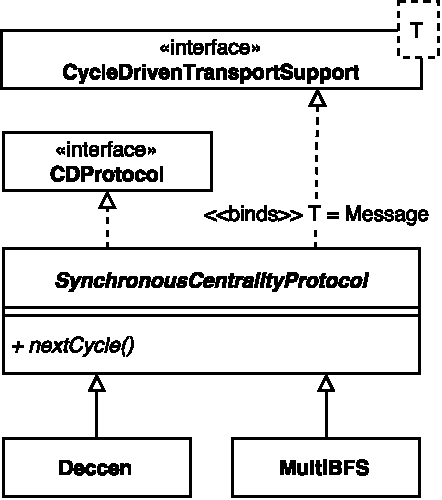
\includegraphics[height=0.31\textheight]{diagram_final.pdf}
\caption{Protocol classes.}
\label{class:protocol:hierarchy}
\end{figure}

Protocol classes are organized as shown in figure \ref{class:protocol:hierarchy}. Both \texttt{Deccen} and \texttt{MultiBFS} extend the abstract class \texttt{SynchronousCentralityProtocol}, which provides an implementation the \texttt{Cycle\-Based\-Transport\-Support<Message>} interface and declares the \texttt{nextCycle} method of the \texttt{CDProtocol} PeerSim interface \texttt{abstract}.

\subsubsection{Messages}
The messages exchanged by the protocols during the simulation are instances of the \texttt{Message} class. This class provides factory methods to generate \mdisc{} and \mrep{} message objects that follow the conventions used in the definition of the algorithms. 

\subsubsection{\deccen{} protocol implementation}

The \texttt{Deccen} class implements a \deccen{} node in the simulator. A node state consists of the shortest path information it collects and of the reports it has handled during the execution:
\begin{minted}{text}
public class Deccen extends SynchronousCentralityProtocol {
  private static class ShortestPathData {
    public final int count;
    public final int length;

    public ShortestPathData(int count, int length) { ... }
  }

  private static class OrderedPair<T1,T2> {
    public final T1 first;
    public final T2 second;

    public OrderedPair(T1 first, T2 second) { ... }
    ...
  }
  ...
  private Map<Node,ShortestPathData> shortestPathMap;
  private Set<OrderedPair<Long,Long>> handledReports;
  ...
  public void nextCycle(Node self, int protocolID) { ... }
  ...
}
\end{minted}
Whenever new \mdisc{} messages are received, additional information about the number and length of shortest paths toward a particular source becomes available: this information is stored in the \texttt{shortestPathMap} structure by adding a new \texttt{ShortestPathData} entry paired with the source of the discovery. Since the algorithm computes all the centrality indices, it stores both the distance from the source and the number of different paths counted. Reports about a source--destination pair $(s,t)$ are tracked by storing the \texttt{handledReports} set an \texttt{Ordered\-Pair} of \texttt{Node} IDs (which are \texttt{long} integers in \peersim{}).

The implementation of \texttt{nextCycle} simply executes the actions described in section \ref{deccen:step}:
\begin{minted}{text}
public void nextCycle(Node self, int protocolID) {
  Map<Node,List<Message>> discoveryMap =
      new HashMap<Node,List<Message>>();
  List<Message> reportList = new LinkedList<Message>();
  parseIncomingMessages(discoveryMap, reportList);
  if (!discoveryMap.isEmpty())
    processDiscoveryMessages(self, protocolID, discoveryMap);
  if (!reportList.isEmpty())
    processReportMessages(self, protocolID, reportList);
}
\end{minted}

\subsubsection{\multibfs{} protocol implementation}

The state of a \multibfs{} node consists of a \texttt{Map} to keep track of the various visits that are performed by the source nodes during the algorithm execution:

\begin{minted}{text}
public class MultiBFS extends SynchronousCentralityProtocol {
  private static class VisitState {
    ...
  }
  ...
  private Map<Node, VisitState> activeVisits;
  private Set<Node> completed;
  ...
  public void nextCycle(Node self, int protocolID) { ... }
  ...
  public boolean isWaiting(Node source) { ... }
  public boolean isActive(Node source) { ... }
  public boolean isCompleted(Node source) { ... }
}
\end{minted}
Recall that the state of a node is parametric with respect to each source of a visit. The state is \swait{\texttt{s}} if the \texttt{Node} instance \texttt{s} does not appear as key in the \texttt{activeVisits} map and neither is contained in the \texttt{completed} set; this is the initial state for any source since both structures are empty at the start of the protocol. When a node is in state \sact{\texttt{s}} an entry with key \texttt{s} is present in the \texttt{activeVisits} map. After a node has reported back to all the predecessors, it changes state \scomp{\texttt{s}} by removing the mapping from \texttt{activeVisits} and inserting \texttt{s} in the \texttt{completed} set.

Entries in the \texttt{activeVisits} map are used to store data while a node is in the ``active'' phase. A \texttt{VisitState} object is used to keep track of the predecessors and children sets, and to incrementally compute the values to be reported to the predecessor nodes:
\begin{minted}{text}
private static class VisitState {
  public Set<Node> predecessors;
  public Set<Node> siblings;
  public Set<Node> children;
  public int distanceFromSource;
  public int timestamp;
  public int sigma;
  public long contributionSC;
  public double contributionBC;
  ...	
  public void accumulate(
      Node child, double bcc, long scc, int numSP) { ... }
}
\end{minted}
The \texttt{accumulate} method updates the local contributions of the source by applying the recursive relations \eqref{eq:th:contrib:bc} and \eqref{eq:th:contrib:sc}, and it's invoked whenever a child node sends a report.

Finally, the \texttt{nextCycle} method follows the specification given in section \ref{multibfs:step}:
\begin{minted}{text}
public void nextCycle(Node self, int protocolID) {
  Map<Node,List<Message>> discoveryMap =
      new HashMap<Node,List<Message>>();
  List<Message> reportList = new LinkedList<Message>();
  parseIncomingMessages(discoveryMap, reportList);
  if (!discoveryMap.isEmpty())
    processDiscoveryMessages(self, protocolID, discoveryMap);
  if (!reportList.isEmpty())
    processReportMessages(reportList);
  reportNewCompleted(self, protocolID);
}
\end{minted}
Messages are parsed and handled by type, then active visits for which all child nodes have reported are finalized with the \texttt{reportNewCompleted} method by integrating the contributions in the centrality accumulators and reporting the relevant data to each predecessor.

\bibliography{p2pbiblio}{}
\bibliographystyle{natbib_ita}
\end{document}
